\documentclass[nooutcomes,handout]{ximera}
%% handout
%% space
%% newpage
%% numbers
%% nooutcomes

%I added the commands here so that I would't have to keep looking them up
%\newcommand{\RR}{\mathbb R}
%\renewcommand{\d}{\,d}
%\newcommand{\dd}[2][]{\frac{d #1}{d #2}}
%\renewcommand{\l}{\ell}
%\newcommand{\ddx}{\frac{d}{dx}}
%\everymath{\displaystyle}
%\newcommand{\dfn}{\textbf}
%\newcommand{\eval}[1]{\bigg[ #1 \bigg]}

%\begin{image}
%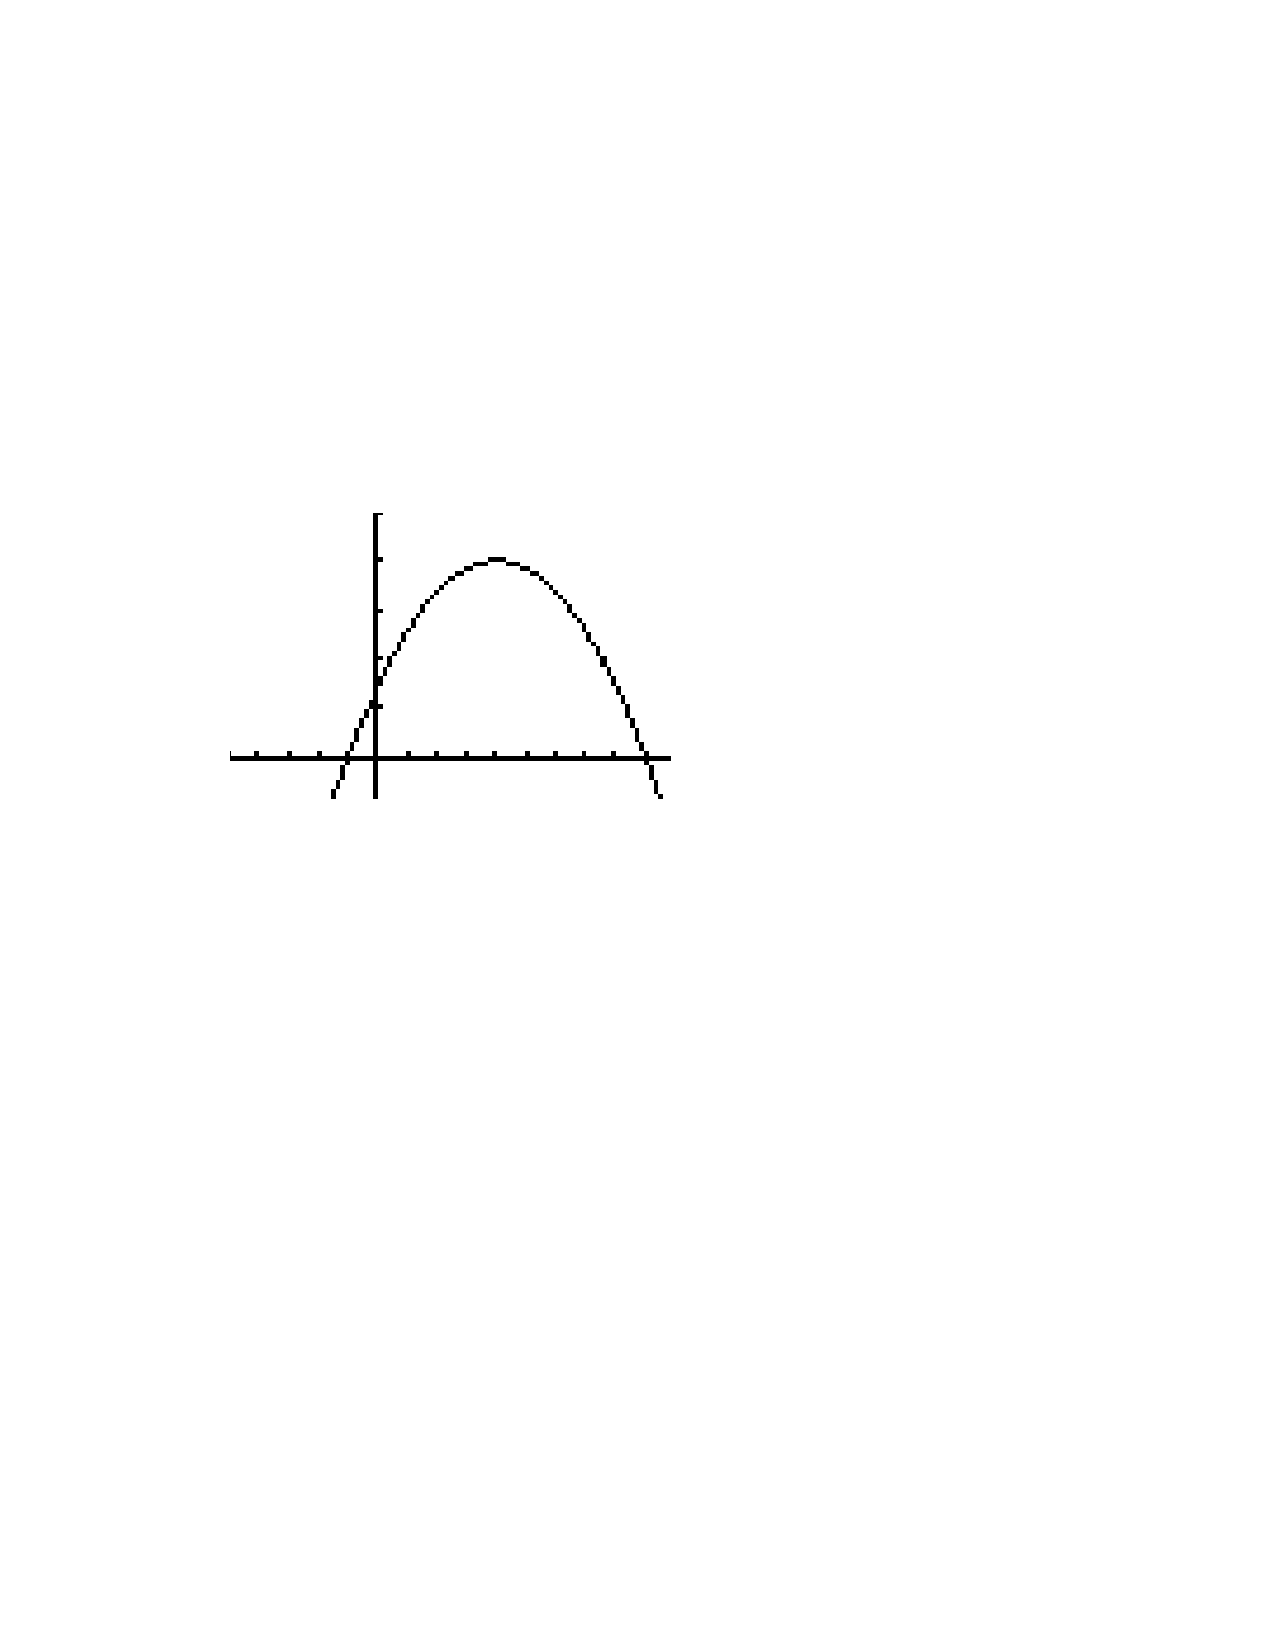
\includegraphics[trim= 170 420 250 180]{Figure1.pdf}
%\end{image}

\usepackage{fullpage}

\newcommand{\RR}{\mathbb R}
\renewcommand{\d}{\,d}
\newcommand{\dd}[2][]{\frac{d #1}{d #2}}
\renewcommand{\l}{\ell}
\newcommand{\ddx}{\frac{d}{dx}}
\newcommand{\dfn}{\textbf}
\newcommand{\eval}[1]{\bigg[ #1 \bigg]}

\usepackage{multicol}

\renewenvironment{freeResponse}{
\ifhandout\setbox0\vbox\bgroup\else
\begin{trivlist}\item[\hskip \labelsep\bfseries Solution:\hspace{2ex}]
\fi}
{\ifhandout\egroup\else
\end{trivlist}
\fi} %% we can turn off input when making a master document

\title{4.1 Maxima and Minima}  

\begin{document}
\begin{abstract}		\end{abstract}
\maketitle

%problem1
\begin{problem}
Determine whether the following statements are true or false and give either an explanation or a counterexample.

	\begin{enumerate}
	
	%part a
	\item  The function $f(x) = \sqrt{x}$ has a local maximum on the interval $[0,1]$.
		\begin{freeResponse}
		False.  Since $\sqrt{x}$ is increasing over the entire region $[0,1]$, the only candidate for a local maximum would be $x=1$.  But by definition, endpoints are never local extrema.  So $f(x) = \sqrt{x}$ has no local maximum on the interval $[0,1]$.
		\end{freeResponse}	
		
		
		
	%part b
	\item  If a function has an absolute maximum value on a closed interval, then the function must be continuous on that closed interval.  
		\begin{freeResponse}
		False.  Consider the following graph for a counterexample.  The function has an absolute maximum on the interval $[2,10]$, but it is not continuous over the entire interval.
		
		\begin{image}
		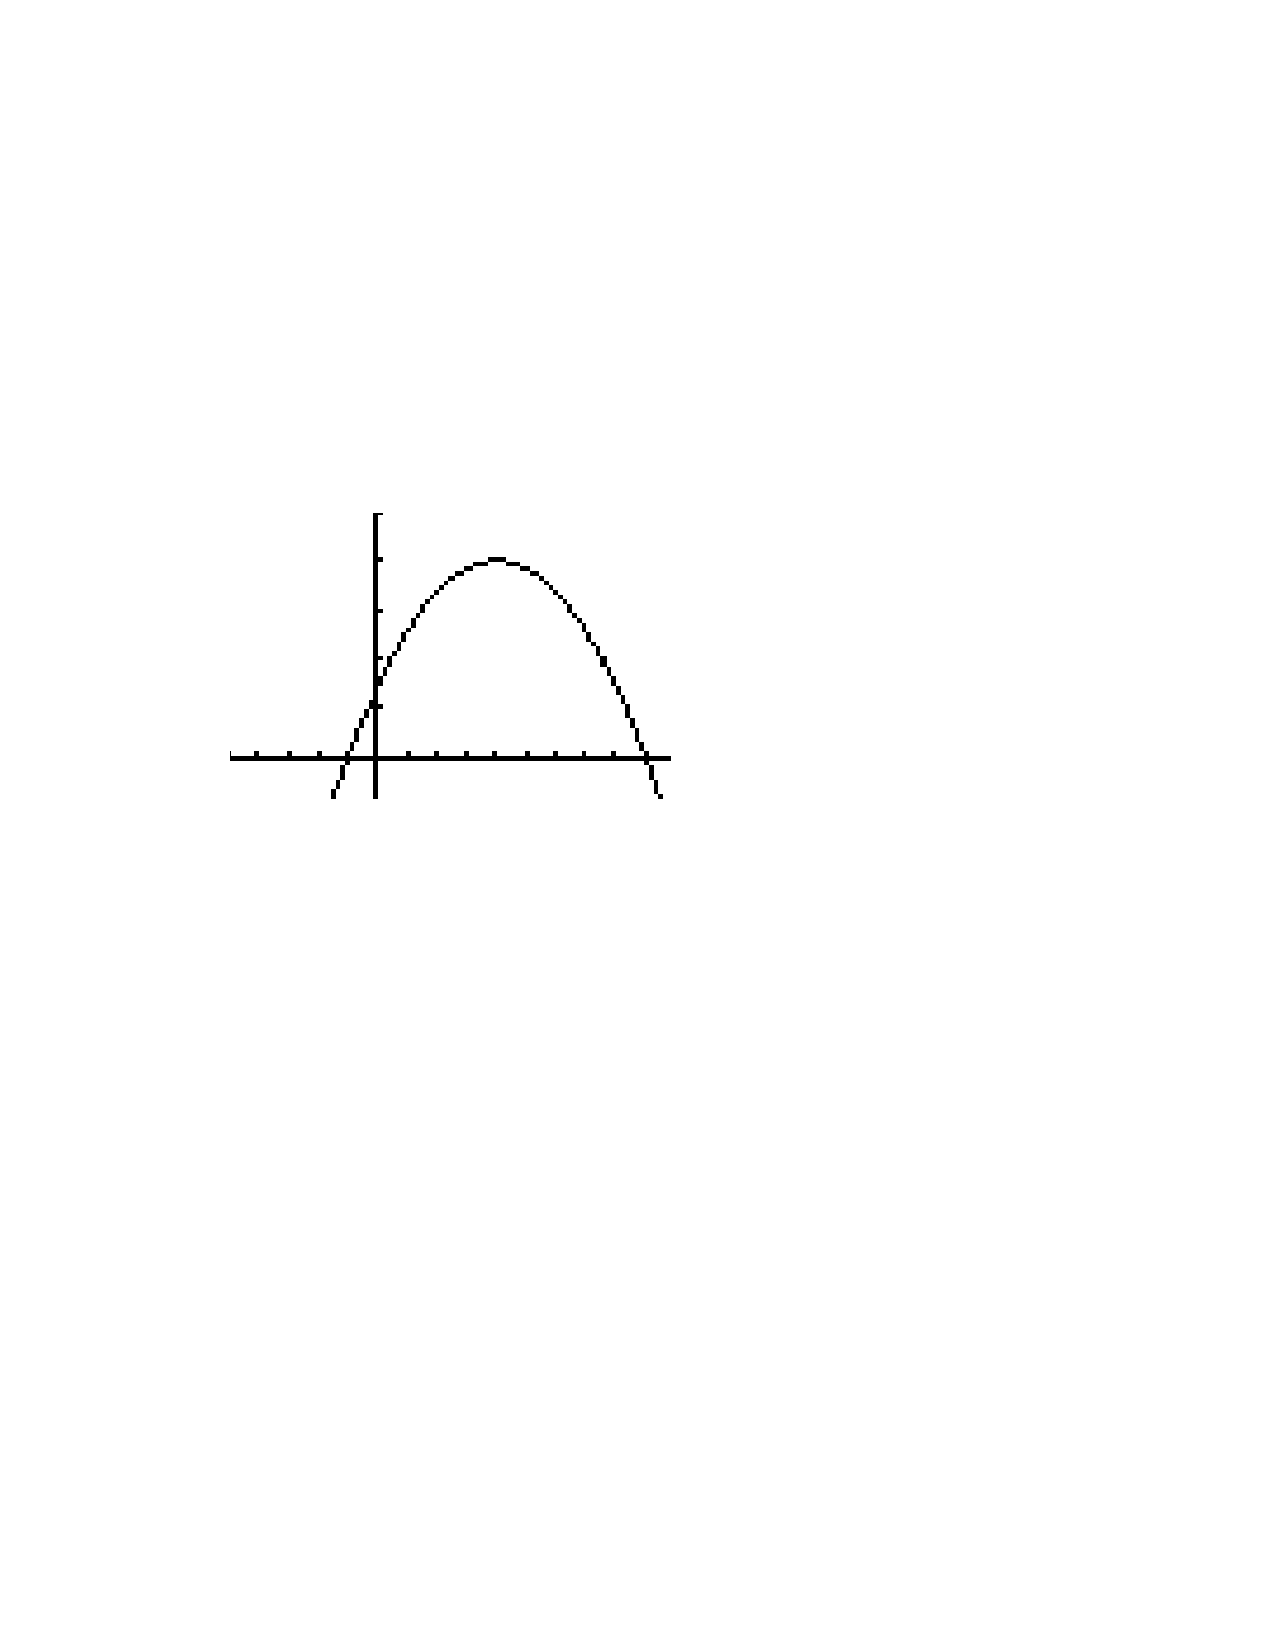
\includegraphics[trim= 170 380 250 180]{Figure1.pdf}
		\end{image}
		
		It is worth noting though that the converse to the original statement is true.  i.e., if a function is continuous on a closed interval then it obtains an absolute maximum value on that closed interval.

		\end{freeResponse}	
		
		
		
	%part c
	\item  If $f'(2)=0$, then $x=2$ is either a local maximum or local minimum of $f$.
		\begin{freeResponse}
		False.  Consider $f(x) = (x-2)^3$.  $f'(x) = 3(x-2)^2$, and so $f'(2) = 0$.  But we can see by looking at the graph of $f$ that $x=2$ is not a local extreme value for $f$.
		
		\begin{image}
		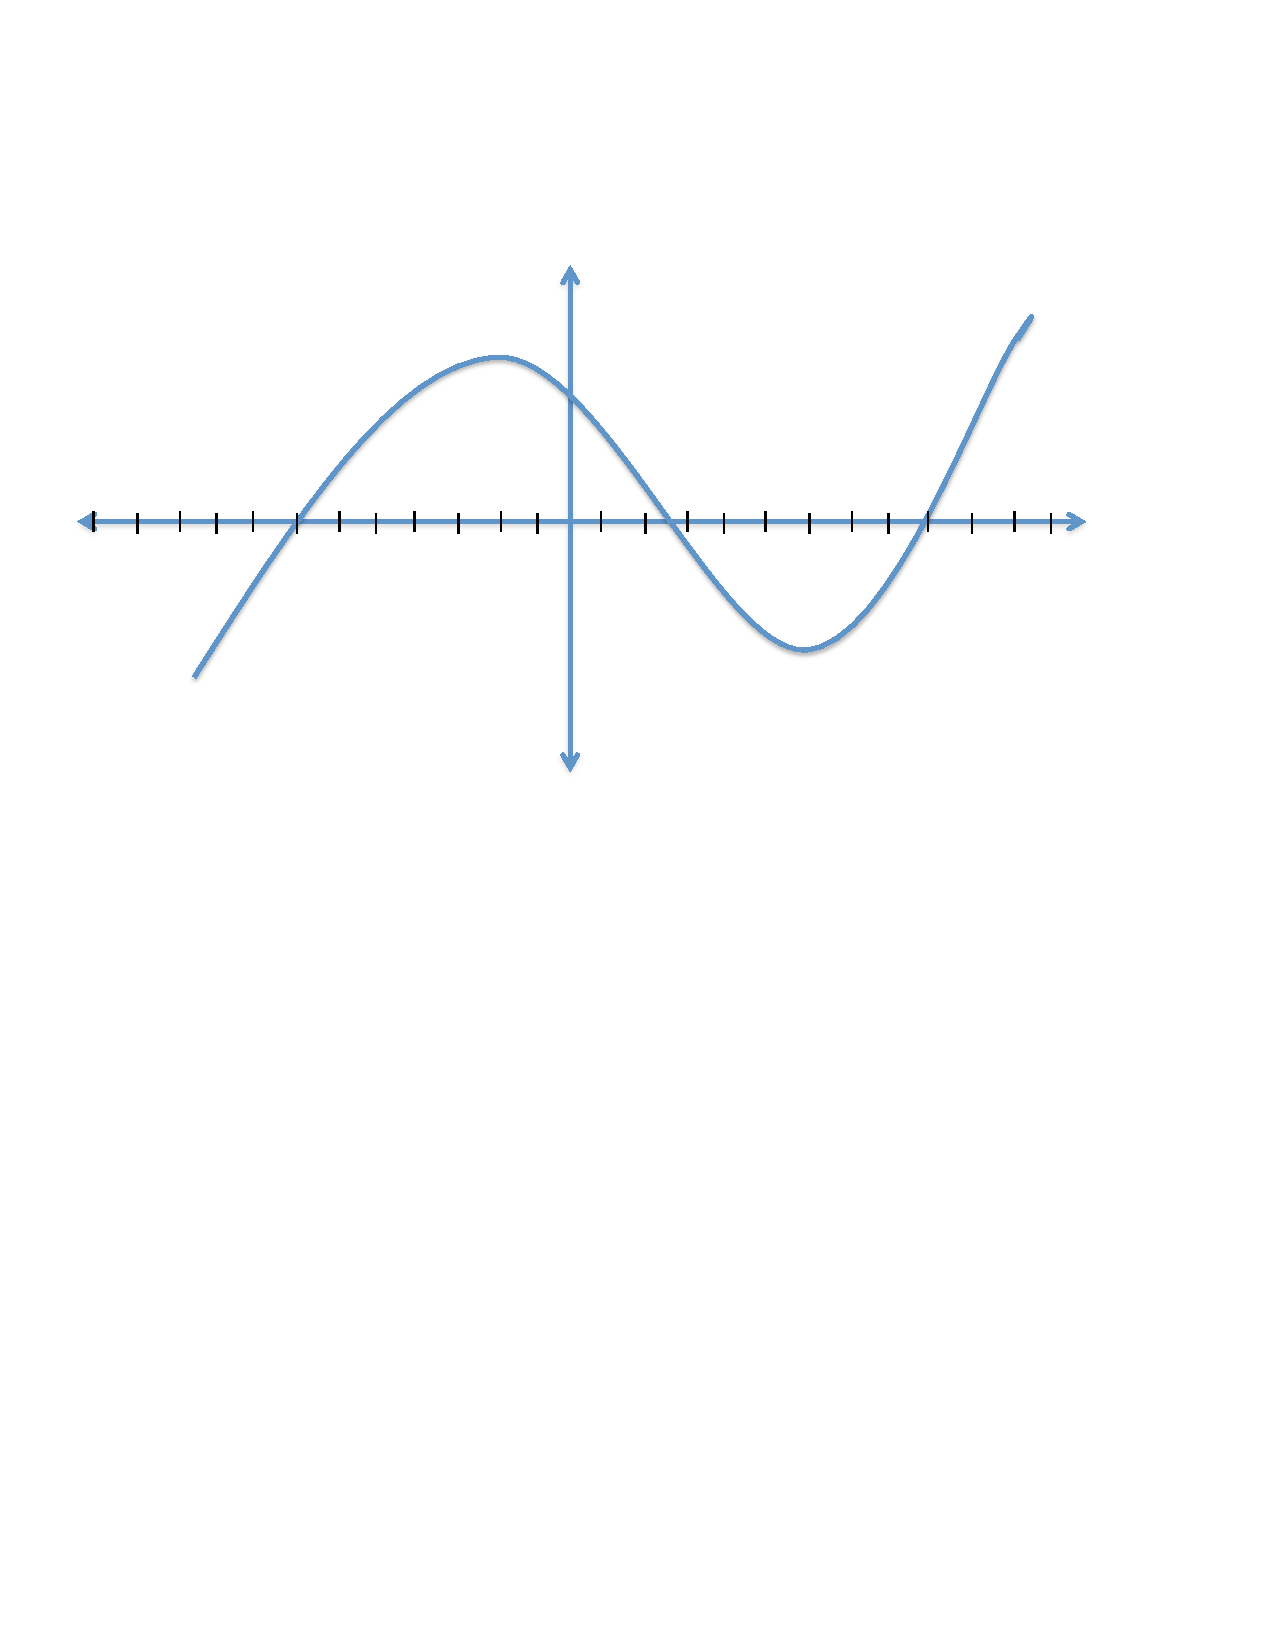
\includegraphics[trim= 100 430 250 180]{Figure2.pdf}
		\end{image}
		
		\end{freeResponse}	
		
		
		
	%part d
	\item  Absolute extreme values on a closed interval always occur at a critical point or an endpoint of the interval.
		\begin{freeResponse}
		True.  That pretty much follows directly from the Local Extreme Value Theorem.  All absolute extrema must either be local extrema or endpoints.  And by the Local Extreme Value Theorem, all local extrema must be critical points of the function.  
		\end{freeResponse}	
		
		
		
	\end{enumerate}
		
\end{problem}	
		




%problem 2
\begin{problem}
For each of the points in the domain of $f$ identified on the graph below, determine if the function $f$ has a critical point, a local max or min, and/or an absolute max or min at that point.

	\begin{center}
	\begin{image}
	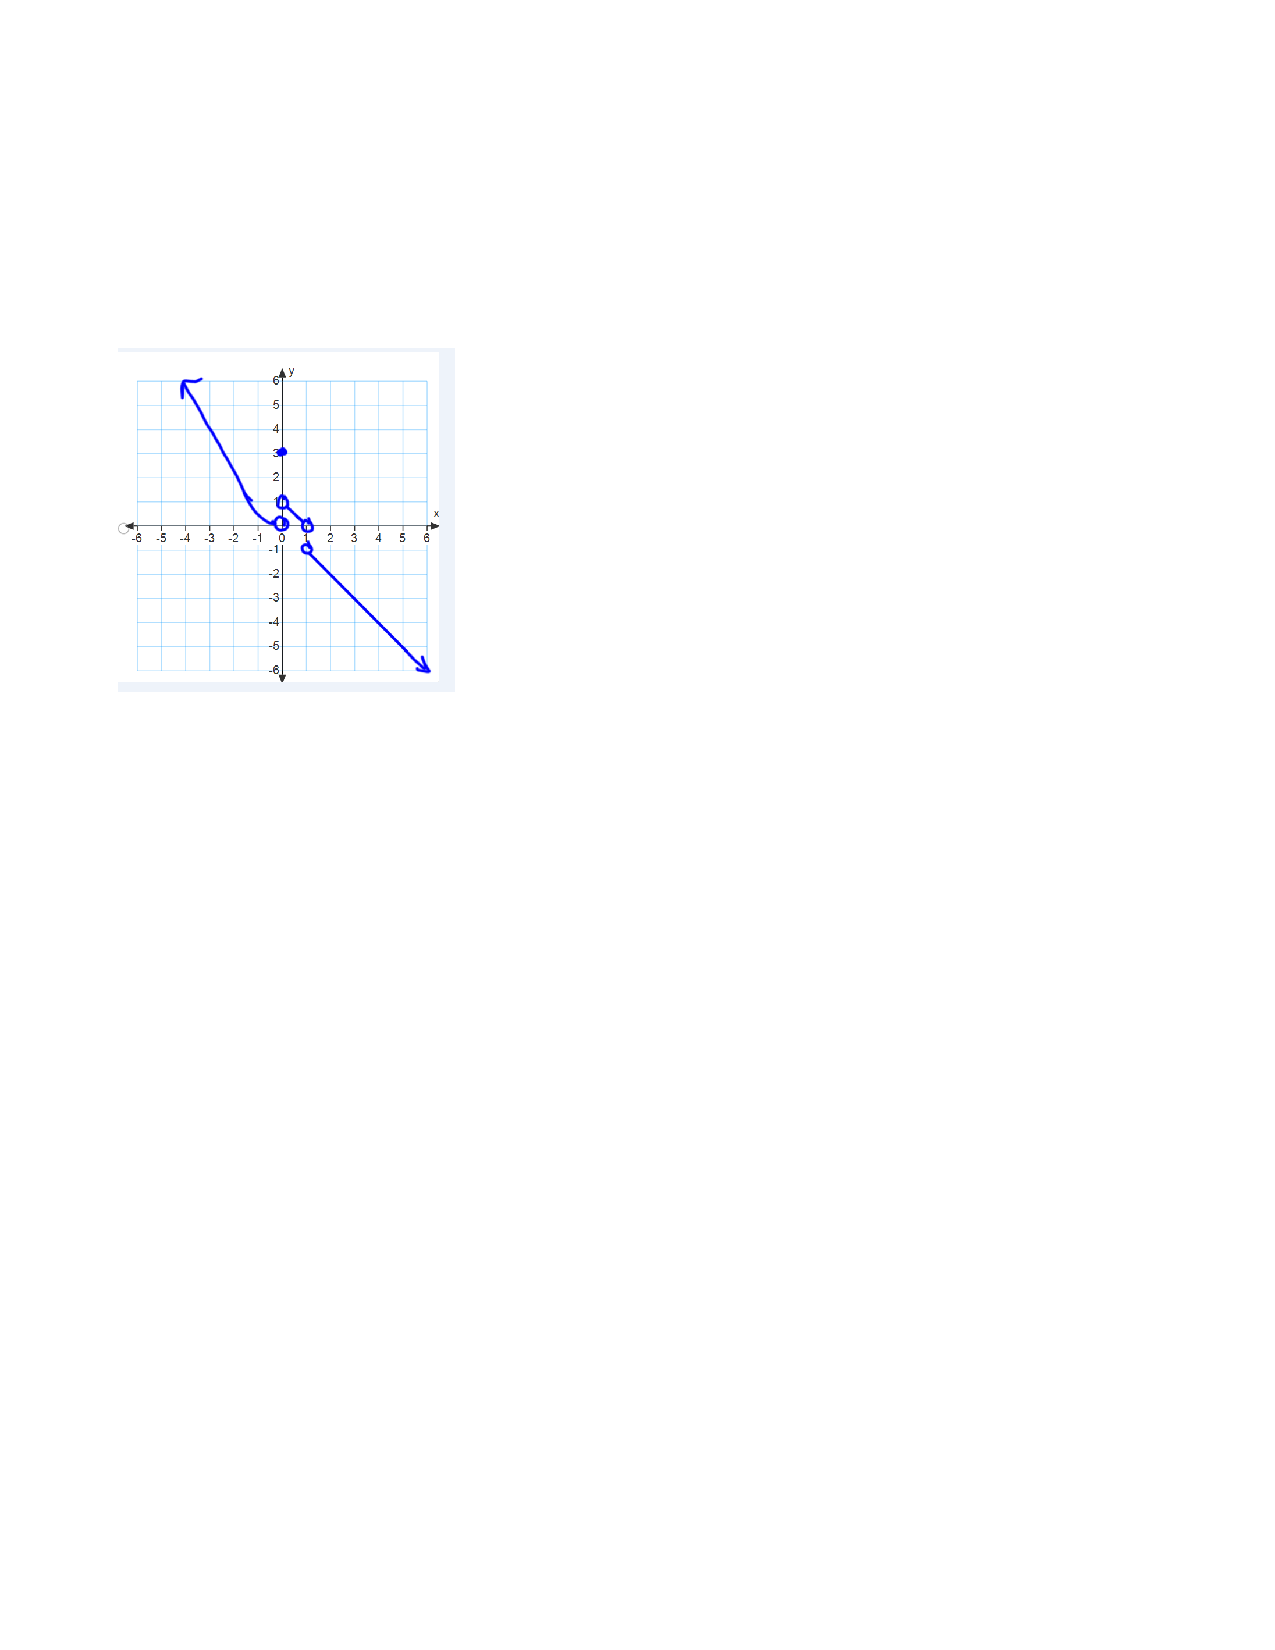
\includegraphics[trim= 20 430 250 200]{Figure3.pdf}
	\end{image}
	\end{center}	
	
		\begin{freeResponse}
(a) The function $f$ has an absolute maximum at $x=a$

(p) The function $f$ has a critical point and an absolute maximum/local maximum at $x=p$.  

(q) The function $f$ has a critical point and a local minimum at $x=q$.

(r) The function $f$ has a critical point and a local maximum at $x=r$

(s) The derivative of $f$ does not exist at $x=s$ because the function $f$ has a corner at $x=s$.  The function has a critical point and a local minimum at $x=s$.

(t) The function $f$ has a critical point but not a local maximum or minimum at $x=t$.

(b) The function $f$ does not have an absolute or local max or min at $x=b$.
		\end{freeResponse}	
		
\end{problem}






%problem 3
\begin{problem}
Find the critical points of $f$ on the given interval, and determine the absolute extreme values of $f$ on the interval.
		\begin{enumerate}
		
			%part a
			\item  $f(x) = x \sqrt{2-x^2}$ on $[ -\sqrt{2}, \sqrt{2} ]$.
				
				\begin{freeResponse}
				First note that $f$ is continuous on this closed interval, and so it must attain a maximum and minimum value on the interval $[-\sqrt{2}, \sqrt{2}]$.
				\begin{align*}
				f'(x) &= \sqrt{2-x^2} + x \left( \frac{1}{2 \sqrt{2-x^2}} (-2x) \right) \\
				&= \sqrt{2-x^2} - \frac{x^2}{\sqrt{2-x^2}} \\
				&= \frac{2-x^2-x^2}{\sqrt{2-x^2}} \\
				&= \frac{2(1-x^2)}{\sqrt{2-x^2}}
				\end{align*}
				
				Critical points of $f$ occur where $f'(x) = 0$ or where $f'(x)$ does not exist.  Solving $f'(x) = 0$ yields that $2(1-x^2) = 0$, or $x = \pm 1$.  $f'(x)$ does not exist when $2-x^2 \leq 0$.  But since we are restricting to the interval $[-\sqrt{2}, \sqrt{2}]$, the only points where $f'(x)$ does not exist are the endpoints $\pm \sqrt{2}$.  
				
				So the critical points of $f$ in the interval $[-\sqrt{2}, \sqrt{2}]$ are $x = \pm 1$.  The points $x = \pm \sqrt{2}$ technically are not critical points since they are the endpoints of the domain of $f$.  In any case, $f$ must attain its maximum and minimum values in this set $x = \pm 1, \pm \sqrt{2}$.  So we compute
				$$ f(-\sqrt{2}) = 0 = f(\sqrt{2}) $$
				$$ f(1) = 1 \sqrt{2-1} = \sqrt{1} = 1$$
				$$ f(-1) = -1 \sqrt{2-(-1)^2} = -1 $$
				
				Thus, $f$ has a maximum value of $1$ (obtained at $x= 1$) and a minimum value of -1 (obtained at $x= -1 $) over the interval $[-\sqrt{2}, \sqrt{2}]$.
				\end{freeResponse}
				
				
				
			%part b
			\item  $f(x) = x^3 e^{-x}$ on $[-1,5]$.
			
				\begin{freeResponse}
				First note that $f$ is continuous on this closed interval, and so it must attain a maximum and minimum value on the interval $[-1,5]$.
				\begin{align*}
				f'(x) &= 3x^2 e^{-x} + x^3(-e^{-x}) \\
				&= x^2 e^{-x} (3-x)
				\end{align*}
				
				Notice that $f'(x)$ always exists, and so all of the critical points of $f$ occur when $f'(x)=0$.  Solving this equation:
				$$ x^2 e^{-x} (3-x) = 0 $$
				$$ x^2 (3-x) = 0 $$
				$$ x = 0 \qquad \text{or} \qquad x=3 $$
				
				Since both critical points are in the given interval, we need to consider the points $x=-1,0,3,5$.
				$$ f(-1) = -e $$
				$$ f(0) = 0 $$
				$$ f(3) = 27e^{-3} $$
				$$ f(5) = 125 e^{-5} $$
				
				Since $-e$ is the only negative value, the minimum value of $f$ over the interval is $-e$.  Since $e^3 < 27$, $27e^{-3} > 1$.  But $e^5 > 125$, and so $125e^{-5} < 1$.  Thus the maximum value of $f$ over the interval is $27e^{-3}$.  
		
				\end{freeResponse}
				
				
				
			%part c
			\item  $f(x) = x \ln \left( \frac{x}{5} \right)$ on $[0.1, 5]$.
			
				\begin{freeResponse}
				First note that $f$ is continuous on this closed interval, and so it must attain a maximum and minimum value on the interval $[0.1,5]$.
				\begin{align*}
				f'(x) &= \ln \left( \frac{x}{5} \right) + x \cdot \frac{5}{x} \cdot \frac{1}{5} \\
				&= \ln \left( \frac{x}{5} \right) + 1
				\end{align*}
				
				Notice that $f'(x)$ exists for all values in $[0.1,5]$, and so all of the critical points of $f$ occur when $f'(x)=0$.  Solving this equation:
				$$ \ln \left( \frac{x}{5} \right) + 1 = 0 $$
				$$ \ln \left( \frac{x}{5} \right) = -1 $$
				$$ \frac{x}{5} = e^{-1} $$
				$$ x = 5e^{-1} = \frac{5}{e} $$
				
				Since $1 < \frac{5}{e} < 2$, $\frac{5}{e}$ is in the given interval.  So we need to consider the points $x = \frac{1}{10}, \frac{5}{e}, 5$.
				$$ f \left( \frac{1}{10} \right) = \frac{1}{10} \ln \left( \frac{1}{50} \right)  = \frac{1}{10} \left( \ln 1 - \ln 50 \right) = -\frac{1}{10} \ln 50 $$
				$$ f \left( \frac{5}{e} \right) = \frac{5}{e} \ln \left( \frac{1}{e} \right) = - \frac{5}{e} $$
				$$ f(5) = 5 \ln 1 = 0 $$
				
				Since the first two values are negative, $0$ is the maximum value of $f$ on $[0.1,5]$.  Also, since $e^{10} > 50$, $\ln 50 < 10$ and therefore $-1 < -\frac{1}{10} \ln 50$.  But clearly $\frac{-5}{e} < -1$, and so $- \frac{5}{e}$ is the minimum value of $f$ on $[0.1, 5]$.  
				
				
		
				\end{freeResponse}
				
				
				
			\end{enumerate}

		
		
		

\end{problem}
	
			
			

%problem 4
\begin{problem}
All rectangles with an area of $64$ inches squared have a perimeter given by $P(x)=2x+\frac{128}{x}$, where $x$ is the length of one side of the rectangle in inches.  Find the absolute minimum value of the perimeter function.  What are the dimensions of the rectangle with minimum perimeter?   
		\begin{freeResponse}
		First note that the domain for $P(x)$ is $(0,\infty)$.  To find the critical points of $P$, we solve the equation $P'(x) = 0$:
		$$ P'(x) = 2 - \frac{128}{x^2} := 0 $$
		$$ \frac{128}{x^2} = 2 $$
		$$ 2x^2 = 128 $$
		$$ x^2 = 64 $$
		$$ x = \pm 8 $$
		but since we must have $x>0$, our only critical point is $x=8$.  Notice that for $x \in (0,8)$, $P'(x) < 0$, and for $x \in (8, \infty)$, $P'(x) > 0$.  Thus $x=8$ is a local minimum.  But since $P$ is decreasing over the entire interval $(0,8)$ and increasing over the entire interval $(8,\infty)$, $x=8$ must be an absolute minimum.
		
		Hence, the absolute minimum perimeter is $P(8) = 16 + \frac{128}{8} = 16 + 16 = 32$ inches.  Since the dimensions of such a rectangle are $8$ inches by $8$ inches, a rectangle of minimum perimeter is a square.
		\end{freeResponse}
			
			
		
\end{problem}






%problem5
\begin{problem}
In each problem, sketch a graph of a function meeting the given critera.
\begin{enumerate}
	%part a
	\item Sketch a possible graph of a function which is continuous on an open interval $(-1,5)$ but does not have an absolute maximum or minimum.
	\begin{freeResponse} \hfil
	\begin{image}
	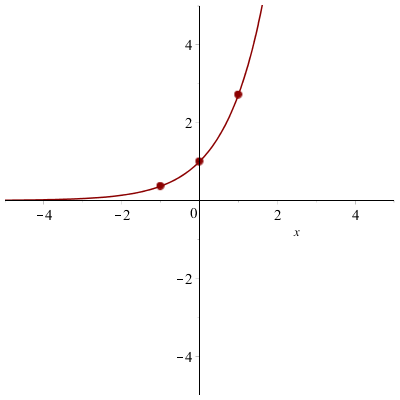
\includegraphics[scale=.5]{Figure5.png}
	\end{image}	
	\end{freeResponse}
	
	%part b
	\item Sketch a possible graph of a function with an absolute minimum, a local maximum and a local minimum, but no absolute maximum on the interval $[-4,5]$.
	\begin{freeResponse} \hfil
	\begin{image}
	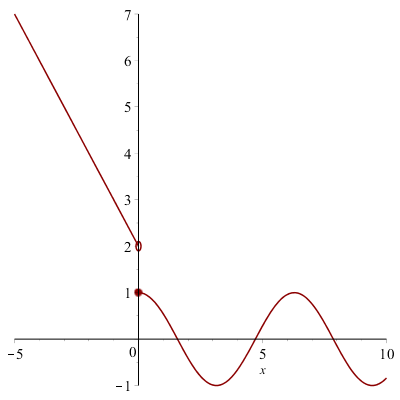
\includegraphics[scale=.4]{Figure6.png}
	\end{image}	
	\end{freeResponse}
	
	%part c	
	\item Sketch a possible graph of a function, $f$, with a local maximum at $2$, and $f'(2)$ is undefined.
	\begin{freeResponse} \hfil
	\begin{image}
	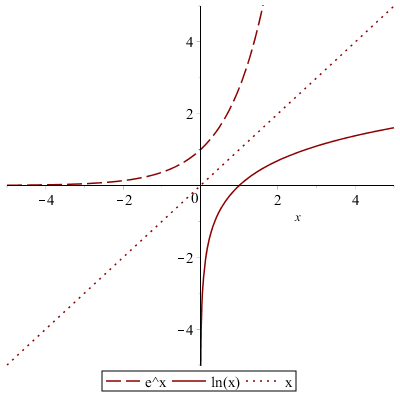
\includegraphics[scale=.4]{Figure4.png}
	\end{image}	
	\end{freeResponse}
	
	%part d	
	 \item Sketch a possible graph of a function $f$, continuous on $[1,4]$ with the following properties: $f'(x)=0$ for $x=2$ and $x=3$; $f$ has an absolute minimum at $x=4$; $f$ has an absolute maxmimum at $x=3$, and $f$ has a local minimum at $x=2$.
		\begin{freeResponse} \hfil
	\begin{image}
	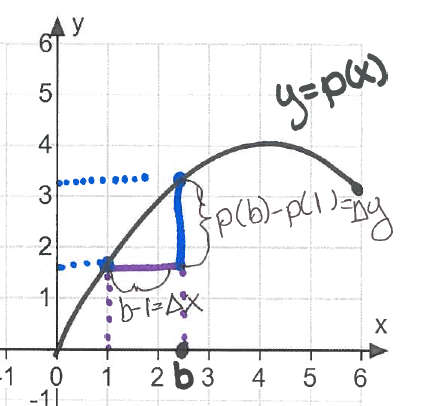
\includegraphics[scale=.5]{Figure7.png}
	\end{image}	
	\end{freeResponse} 
	 
	 \end{enumerate}
	 \end{problem}






\end{document} 


















